\chapter{أكسدة الألكينات واختزالها}\label{ch:b2:alkene-redox}

يأتي غراء الإيبوكسي الثنائي المكوّن في أنبوبين: يحوي أحدهما جزيئات تنتهي
بحلقات \omterm{def:b2:alkene-redox:epoxide}{إيبوكسيد}، وهي حلقات ثلاثية من كربونين وأكسجين؛ ويحوي الآخر
أمينًا. وعند الخلط تنفتح الحلقات المتوترة الواحدة تلو الأخرى فيتصلب العجين
في شبكة صلبة. والألكينات هي المادة الأولية لمثل هذه الحلقات، وللكحولات
الموضوعة حيث لا تضعها قاعدة ماركوفنيكوف أبدًا، وللديولات ذات
الهندسة المختارة، وللشظايا الصغيرة التي كانت تُخبر الكيميائيين بموضع الرابطة
المزدوجة في الجزيء. ويضيف هذا الفصل إلى الإضافات المحبة للإلكترونات في
مجلد السنة الأولى التفاعلات التي تختزل الرابطة المزدوجة أو تؤكسدها، 
والكيمياء الفراغية التي يفرضها كل منها.

\begin{recall}
مجلد السنة الأولى: الإضافات المحبة للإلكترونات، وقاعدة ماركوفنيكوف، وأيونات الهالونيوم،
والإضافات المتزامنة والمضادة، وإماهة الألكينات، ومستويات أكسدة الكربون،
ومانحات الهيدريد، والانتقائية الكيميائية، ومركبات ميزو والخلائط الراسيمية،
والتفاعلات النوعية فراغيًا. و\cref{ch:b2:catalytic-cycles}: دورة الهدرجة بحفاز
ويلكنسون.
\end{recall}

\begin{omfigure}
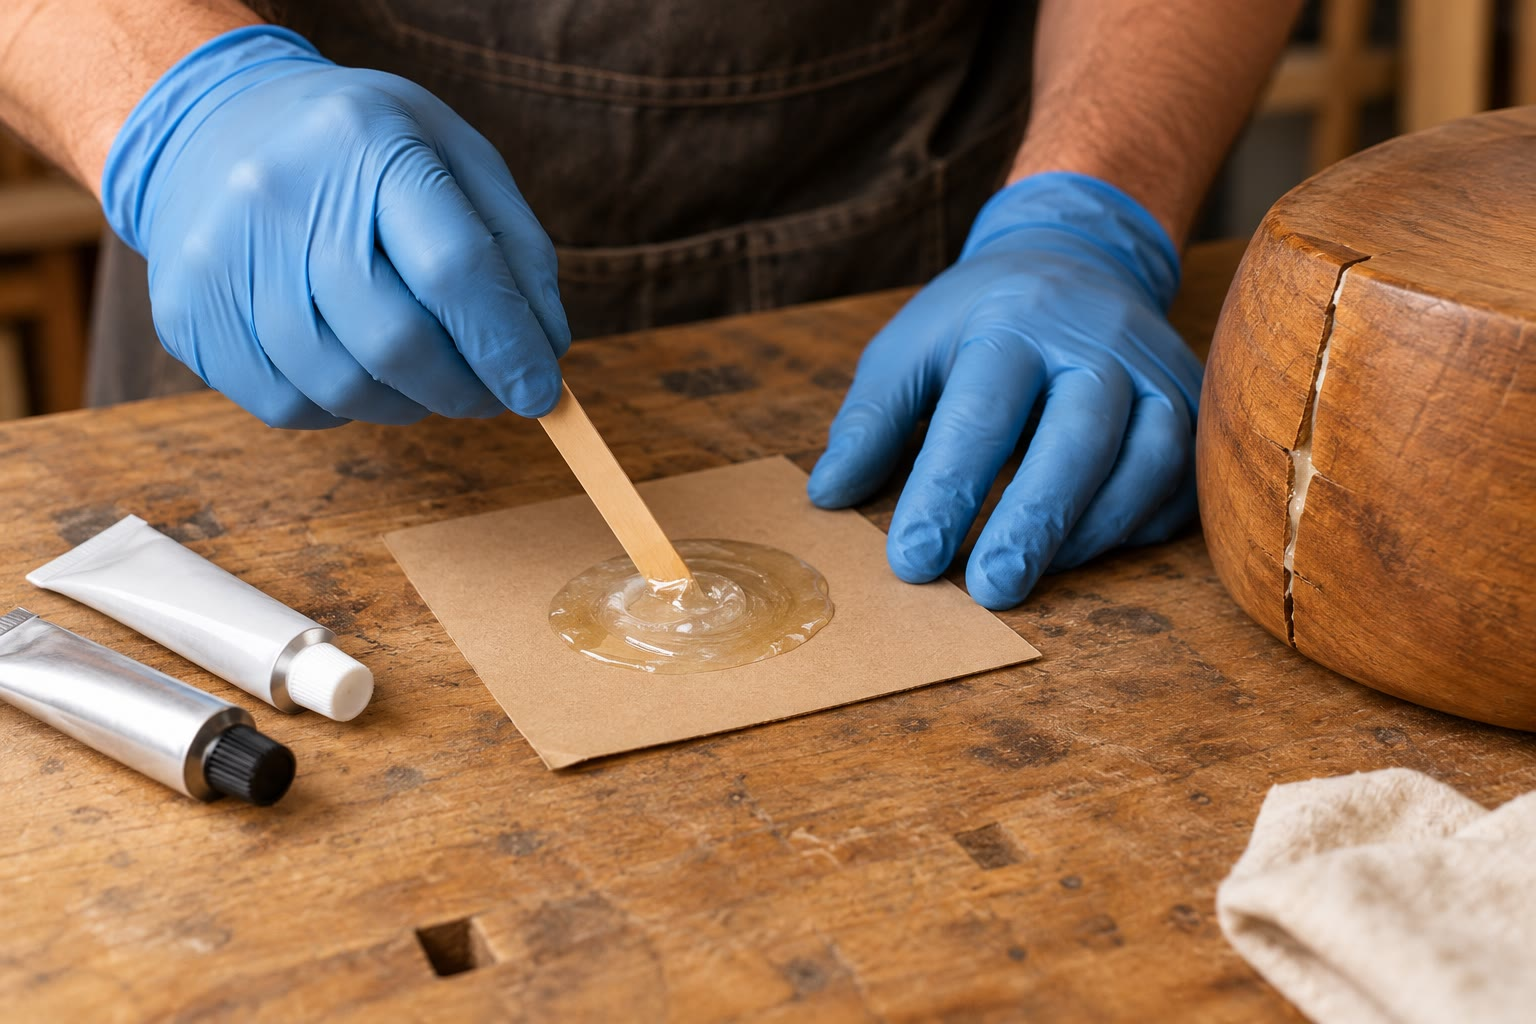
\includegraphics[width=0.6\linewidth]{images/book3/ai/b2-21-epoxy.jpg}

{\small خلط غراء إيبوكسي ثنائي المكوّن: يتفاعل الراتنج، بمجموعاته الإيبوكسيدية، 
والمصلِّد، وهو أمين، حالما يلتقيان؛ فتنفتح الحلقات وتربط الجزيئات
في شبكة صلبة.}
\end{omfigure}

\section{الهدرجة الحفزية}

\begin{definition}[الهدرجة الحفزية]\label{def:b2:alkene-redox:hydrogenation}
\emph{الهدرجة الحفزية}\index{هدرجة حفزية} تضيف ثنائي الهيدروجين عبر
رابطة متعددة بوجود حفاز: فلز مجزأ تجزيئًا دقيقًا (البلاديوم على
الكربون، البلاتين، النيكل) في الحفز غير المتجانس، أو معقد ذواب مثل
حفاز ويلكنسون في الحفز المتجانس.
\end{definition}

على سطح الفلز، يُمسك ثنائي الهيدروجين والألكين كلاهما، وتنكسر الرابطة \ce{H-H}
إلى ذرات هيدروجين سطحية، تنتقل الواحدة تلو الأخرى إلى ذرتي الكربون
في الألكين، الذي يستلقي مسطحًا على الفلز.

\begin{proposition}[الإضافة المتزامنة]\label{prop:b2:alkene-redox:syn-hydrogenation}
تنقل \omterm{def:b2:alkene-redox:hydrogenation}{الهدرجة الحفزية} ذرتي الهيدروجين كلتيهما إلى الوجه نفسه من الرابطة المزدوجة.
والألكاين المهدرج على حفاز بلاديوم مسموم يتوقف عند الألكين، الذي هو
المتماكب (\textit{Z}).
\end{proposition}

\begin{proof}[تعليل]
يرتبط الألكين بالحفاز بأحد وجهيه، ويأتي الهيدروجينان كلاهما من
الحفاز، على ذلك الوجه: إضافة متزامنة. ومع الألكاين، يكون الهيدروجينان المضافان إلى
الرابطة الثلاثية في الجهة نفسها، في وضع cis أحدهما بالنسبة إلى الآخر: الألكين (\textit{Z}). والحفاز
المعطَّل جزئيًا (البلاديوم على كربونات الكالسيوم مع ملح للرصاص والكينولين)
يربط الألكاين بقوة أكبر بكثير من الألكين المتكوّن، الذي يغادر السطح
قبل إضافة ثانية.
\end{proof}

\section{الهيدروبورة--الأكسدة}

\begin{definition}[الهيدروبورة]\label{def:b2:alkene-redox:hydroboration}
\emph{الهيدروبورة}\index{هيدروبورة} تضيف رابطة B--H من بوران عبر
رابطة \ce{C=C}؛ وحين تتبعها أكسدة بفوق أكسيد الهيدروجين القلوي، تحوّل
الألكين إلى كحول تقع مجموعة الهيدروكسيل فيه على الكربون الأقل استبدالًا: وهذا
\emph{توجيه مضاد لماركوفنيكوف}\index{توجيه مضاد لماركوفنيكوف}.
\end{definition}

\begin{omfigure}
\setchemfig{atom sep=1.8em}
\schemestart[][west]
\chemfig{H_3C-[:30]CH=[:-30]CH_2}
\+ \chemfig{H-BH_2}
\arrow{->[إضافة متزامنة]}
\chemfig{H_3C-[:30]CH_2-[:-30]CH_2-[:30]BH_2}
\arrow{->[\ce{H2O2}][\ce{HO-}]}
\chemfig{H_3C-[:30]CH_2-[:-30]CH_2-[:30]OH}
\schemestop
\par\vspace{6pt}

{\small \omterm{def:b2:alkene-redox:hydroboration}{هيدروبورة} البروبين ثم أكسدته. يُضاف البوران في خطوة واحدة، البور إلى
الكربون الطرفي والهيدروجين إلى الكربون الداخلي، وكلاهما على الوجه نفسه؛ وتستبدل الأكسدة
بالبور المجموعة \ce{OH} مع احتفاظ بالترتيب الفراغي. فيتكوّن البروبان-1-ول، لا
البروبان-2-ول الناتج من الإماهة المحفَّزة بالحمض.}
\end{omfigure}

\begin{proposition}[توجيه الهيدروبورة]\label{prop:b2:alkene-redox:hydroboration-regio}
يُضاف البور إلى الكربون الأقل استبدالًا في الرابطة المزدوجة، والهيدروجين إلى الكربون
الأكثر استبدالًا؛ والإضافة متزامنة.
\end{proposition}

\begin{proof}[تعليل]
البور، بمداره p الفارغ، هو المحب للإلكترونات: ففي الحالة الانتقالية الرباعية المراكز
(الكربونان والبور والهيدروجين)، تتكوّن الرابطة مع البور قبل الرابطة C--H بقليل، 
وتنشأ شحنة موجبة جزئية على الكربون الآخر، يحملها الكربون الأكثر استبدالًا
على نحو أفضل؛ ومجموعة البور الضخمة تفضّل أيضًا الطرف الأقل إعاقة. وتتكوّن الرابطتان الجديدتان
كلتاهما على وجه واحد، في خطوة متضافرة: إضافة متزامنة.
\end{proof}

\begin{proposition}[الأكسدة مع الاحتفاظ بالترتيب]\label{prop:b2:alkene-redox:retention}
أكسدة ألكيل بوران بفوق أكسيد الهيدروجين القلوي تستبدل بكل رابطة C--B
رابطة كربون--هيدروكسيل مع الاحتفاظ بالترتيب الفراغي عند الكربون.
\end{proposition}

\begin{proof}[تعليل]
يُضاف أنيون الهيدروبيروكسيد إلى البور؛ ثم تهاجر مجموعة ألكيل من البور إلى
الأكسجين المجاور، بزوج إلكتروناتها، بينما يغادر الهيدروكسيد؛ ويبقي الكربون روابطه
في الجهة نفسها طوال الوقت. ويحرر حلمهة الرابطة B--O الكحول.
\end{proof}

\section{الإيبوكسيدات}

\begin{definition}[الإيبوكسيد]\label{def:b2:alkene-redox:epoxide}
\emph{الإيبوكسيد}\index{إيبوكسيد} (الأوكسيران) إيثر حلقي ذو حلقة ثلاثية من
كربونين وأكسجين واحد. و\emph{الإيبكسدة}\index{إيبكسدة} تحوّل الألكين إلى
إيبوكسيد، عادة بواسطة \emph{حمض بيروكسي}\index{حمض بيروكسي} \ce{RCO3H}، الذي ينقل
ذرة أكسجين واحدة إلى الرابطة المزدوجة.
\end{definition}

\begin{omfigure}
\setchemfig{atom sep=2em}
\schemestart
\chemfig{R-[:30]CH=[:-30]CH-[:30]R}
\+ \chemfig{Ar-C(=[2]O)-O-O-H}
\arrow{->}
\chemfig{[:-60]CH(-[:210]R)*3(-CH(-[:-30]R)-O-)}
\+ \chemfig{Ar-C(=[2]O)-OH}
\schemestop
\par\vspace{6pt}

{\small \omterm{def:b2:alkene-redox:epoxide}{الإيبكسدة} \omterm{def:b2:alkene-redox:epoxide}{بحمض بيروكسي} (Ar: مثلًا مجموعة 3-كلوروفينيل). ينتقل الأكسجين
الطرفي \omterm{def:b2:alkene-redox:epoxide}{لحمض البيروكسي} إلى الرابطة المزدوجة في خطوة واحدة، وتتكوّن الرابطتان C--O
كلتاهما على الوجه نفسه.}
\end{omfigure}

\begin{proposition}[الإيبكسدة النوعية فراغيًا]\label{prop:b2:alkene-redox:epoxidation}
\omterm{def:b2:alkene-redox:epoxide}{الإيبكسدة} \omterm{def:b2:alkene-redox:epoxide}{بحمض بيروكسي} نوعية فراغيًا: فالألكين (\textit{Z}) يعطي \omterm{def:b2:alkene-redox:epoxide}{الإيبوكسيد} cis،
والألكين (\textit{E}) يعطي \omterm{def:b2:alkene-redox:epoxide}{الإيبوكسيد} trans.
\end{proposition}

\begin{proof}
ينتقل الأكسجين في خطوة متضافرة واحدة إلى أحد وجهي الرابطة المزدوجة، التي لا
تدور في أثناء ذلك: فتُحفظ المواضع النسبية للبدائل.
\end{proof}

\begin{proposition}[فتح الإيبوكسيدات]\label{prop:b2:alkene-redox:opening}
يفتح المحب للنواة \omterm{def:b2:alkene-redox:epoxide}{الإيبوكسيد} بالهجوم على أحد الكربونين من الوجه المقابل للأكسجين
(فتح مضاد، مع انقلاب عند ذلك الكربون). وفي الظروف القاعدية، يهاجم الكربون الأقل
إعاقة؛ وفي الظروف الحمضية، الكربون الأكثر استبدالًا.
\end{proposition}

\begin{proof}[تعليل]
توتر الحلقة يجعل كسر الرابطتين C--O سهلًا. ومع محب للنواة قوي وبلا حمض،
يكون الفتح استبدالًا ثنائي الجزيئية، ويُبلغ الكربون الأقل إعاقة بأكبر
سهولة. وفي الحمض يُبرتن الأكسجين؛ فتستطيل الرابطة C--O مع الكربون الأكثر استبدالًا
أكثر من غيرها، لأن ذلك الكربون يحمل الشحنة الموجبة الجزئية الأكبر، وحتى المحب للنواة
الضعيف (الماء، الكحول) يهاجم هناك --- ومن الخلف دائمًا، فيبقى الفتح مضادًا.
\end{proof}

\begin{omfigure}
\setchemfig{atom sep=2em}
\schemestart
\chemfig{[:-60]C(-[:210]H_3C)(-[:150]H_3C)*3(-CH_2-O-)}
\arrow{->[\ce{CH3O-}][\ce{CH3OH}]}[,1.4]
\chemfig{H_3C-C(-[2]CH_3)(-[6]OH)-CH_2-OCH_3}
\schemestop

\medskip
\schemestart
\chemfig{[:-60]C(-[:210]H_3C)(-[:150]H_3C)*3(-CH_2-O-)}
\arrow{->[\ce{CH3OH}][\ce{H+}]}[,1.4]
\chemfig{H_3C-C(-[2]CH_3)(-[6]OCH_3)-CH_2-OH}
\schemestop
\par\vspace{6pt}

{\small فتح 2،2-ثنائي ميثيل أوكسيران بالميثانول. في الأعلى، مع الميثوكسيد: هجوم على
\ce{CH2}، الكربون الأقل إعاقة. وفي الأسفل، في الحمض: هجوم على الكربون الأكثر استبدالًا،
الذي يحمل معظم الشحنة الموجبة \omterm{def:b2:alkene-redox:epoxide}{للإيبوكسيد} المبرتن.}
\end{omfigure}

\section{الهدركسلة الثنائية}

\begin{definition}[الهدركسلة الثنائية]\label{def:b2:alkene-redox:dihydroxylation}
\emph{الهدركسلة الثنائية}\index{هدركسلة ثنائية} تحوّل الألكين إلى 1،2-ديول بإضافة
مجموعة \ce{OH} واحدة إلى كل كربون من الرابطة المزدوجة.
\end{definition}

رباعي أكسيد الأوزميوم، بكمية حفزية مع عامل معيد للأكسدة، والبرمنغنات المخففة الباردة يضيفان
الأكسجينين كليهما عبر إستر حلقي، على وجه واحد: \omterm{def:b2:alkene-redox:dihydroxylation}{هدركسلة ثنائية} متزامنة. أما \omterm{def:b2:alkene-redox:epoxide}{الإيبكسدة}
المتبوعة بالفتح بالماء في الحمض فتعطي الديول المضاد.

\begin{proposition}[الديولات المتزامنة والمضادة]\label{prop:b2:alkene-redox:diols}
من (\textit{Z})-بوت-2-ين، تعطي \omterm{def:b2:alkene-redox:dihydroxylation}{الهدركسلة الثنائية} المتزامنة ميزو-بوتان-2،3-ديول ويعطي
طريق \omterm{def:b2:alkene-redox:epoxide}{الإيبوكسيد} الديولين (2\textit{R}،3\textit{R}) و(2\textit{S}،3\textit{S}) خليطًا راسيميًا؛ ومن
(\textit{E})-بوت-2-ين، تتبادل النتيجتان.
\end{proposition}

\begin{proof}
في (\textit{Z})-بوت-2-ين تقع مجموعتا الميثيل في الجهة نفسها. وإضافة مجموعتي \ce{OH} على وجه واحد
تعطي ديولًا تقع فيه، حين يُكتب في التشكّل المتطابق للرابطة المزدوجة السابقة،
مجموعتا \ce{OH} في جهة ومجموعتا الميثيل في الجهة الأخرى: فيمر مستوي مرآة بين
C2 وC3، وهذا مركب الميزو. أما طريق \omterm{def:b2:alkene-redox:epoxide}{الإيبوكسيد} فيضع مجموعتي \ce{OH} على وجهين متقابلين
(مضادًا): فيضيع مستوي المرآة، والهجوم على أي من كربوني \omterm{def:b2:alkene-redox:epoxide}{الإيبوكسيد} اللاكيرالي،
المتساويين في الاحتمال، يعطي المتماكبين المرآويين بكميتين متساويتين. ومن أجل الألكين (\textit{E}) تغيّر كل
خطوة العلاقة بين مجموعتي الميثيل، فتتبادل النتيجتان.
\end{proof}

\begin{omfigure}
\begin{tikzpicture}[font=\small]
  \begin{scope}
    \draw[thick] (0,0) -- (0,1.2);
    \draw[thick] (0,1.2) -- (-0.7,1.45); \draw[thick] (0,1.2) -- (0.7,1.45);
    \node[anchor=east] at (-0.7,1.45) {\ce{HO}}; \node[anchor=west] at (0.7,1.45) {\ce{CH3}};
    \draw[thick] (0,0) -- (-0.7,0.25); \draw[thick] (0,0) -- (0.7,0.25);
    \node[anchor=east] at (-0.7,0.25) {\ce{HO}}; \node[anchor=west] at (0.7,0.25) {\ce{CH3}};
    \node[anchor=south] at (0,1.25) {\scriptsize H};
    \node[anchor=north] at (0,-0.05) {\scriptsize H};
    \draw[densely dashed, omThm] (-1.6,0.6) -- (1.6,0.6);
    \node at (0,-1.0) {\foreignlanguage{arabic}{متزامنة: ميزو}};
  \end{scope}
  \begin{scope}[xshift=6.5cm]
    \draw[thick] (0,0) -- (0,1.2);
    \draw[thick] (0,1.2) -- (-0.7,1.45); \draw[thick] (0,1.2) -- (0.7,1.45);
    \node[anchor=east] at (-0.7,1.45) {\ce{HO}}; \node[anchor=west] at (0.7,1.45) {\ce{CH3}};
    \draw[thick] (0,0) -- (-0.7,0.25); \draw[thick] (0,0) -- (0.7,0.25);
    \node[anchor=east] at (-0.7,0.25) {\ce{H3C}}; \node[anchor=west] at (0.7,0.25) {\ce{OH}};
    \node[anchor=south] at (0,1.25) {\scriptsize H};
    \node[anchor=north] at (0,-0.05) {\scriptsize H};
    \node[align=center] at (0,-1.1) {\foreignlanguage{arabic}{مضادة: متماكب مرآوي واحد}\\ \foreignlanguage{arabic}{يتكوّن مع صورته المرآوية}};
  \end{scope}
\end{tikzpicture}

{\small البوتان-2،3-ديولان الناتجان من (\textit{Z})-بوت-2-ين، رسم تخطيطي (الرابطة C2--C3
عمودية، والمجموعتان على كل كربون مرسومتان يسارًا ويمينًا). تضع الإضافة المتزامنة مجموعتي
\ce{OH} كلتيهما في الجهة نفسها: مستوي مرآة داخلي (متقطع)، مركب الميزو. وتضعهما الإضافة
المضادة في جهتين متقابلتين: ديول كيرالي، يتكوّن مع متماكبه المرآوي.}
\end{omfigure}

\section{الانشطار التأكسدي}

\begin{definition}[الانشطار التأكسدي]\label{def:b2:alkene-redox:cleavage}
\emph{الانشطار التأكسدي}\index{انشطار تأكسدي} يكسر رابطتي الرابطة المزدوجة \ce{C=C}
كلتيهما ويحوّل كل كربون إلى مجموعة كربونيل أو كربوكسيل. وفي
\emph{التحلل الأوزوني}\index{تحلل أوزوني}، يتفاعل الألكين مع الأوزون ويُفكَّك
الأوزونيد الوسيط في خطوة ثانية، هي المعالجة اللاحقة.
\end{definition}

\begin{proposition}[نواتج التحلل الأوزوني]\label{prop:b2:alkene-redox:ozonolysis}
يشطر \omterm{def:b2:alkene-redox:cleavage}{التحلل الأوزوني} كل رابطة \ce{C=C} إلى مجموعتي \ce{C=O}. ومع معالجة لاحقة مختزلة
(الزنك والحمض، أو كبريتيد ثنائي الميثيل)، يعطي الكربون الحامل لهيدروجين ألدهيدًا؛ ومع
معالجة لاحقة مؤكسدة (فوق أكسيد الهيدروجين)، يعطي حمضًا كربوكسيليًا. والكربون الحامل لمجموعتين
كربونيتين يعطي كيتونًا في الحالتين.
\end{proposition}

\begin{proof}[تعليل]
يُضاف الأوزون إلى الرابطة المزدوجة، ويُعاد ترتيب الوسيط وتنكسر الرابطة C--C، فيعطي
أوزونيدًا ترتبط فيه كل ذرة كربون ألكينية سابقة بذرتي أكسجين. والمعالجة اللاحقة تختزله
إلى مركبين كربونيليين، أو تؤكسد الألدهيدات أكثر. والخطوات الوسيطة
مقبولة هنا.
\end{proof}

\begin{omfigure}
\setchemfig{atom sep=2em}
\schemestart
\chemfig{H_3C-[:30]C(-[:90]CH_3)=[:-30]CH-[:30]CH_3}
\arrow{->[1. \ce{O3}][2. \ce{Zn}, \ce{H+}]}[,1.8]
\chemfig{H_3C-C(=[2]O)-CH_3}
\+
\chemfig{H-C(=[2]O)-CH_3}
\schemestop
\par\vspace{6pt}

{\small \omterm{def:b2:alkene-redox:cleavage}{التحلل الأوزوني} للمركب 2-ميثيل بوت-2-ين مع معالجة لاحقة مختزلة: البروبانون 
والإيثانال. ووصل ذرتي الكربون الكربونيليتين من جديد برابطة مزدوجة يعيد بناء
الألكين.}
\end{omfigure}

\begin{method}[تحديد موضع رابطة مزدوجة]\label{met:b2:alkene-redox:locate-double-bond}
\begin{enumerate}
  \item عدّد الشظايا الكربونيلية \omterm{def:b2:alkene-redox:cleavage}{للتحلل الأوزوني} وعُدّ كربوناتها؛ يجب أن يساوي مجموعها
        كربونات الألكين.
  \item كل كربون \ce{C=O} كان كربونًا ذا رابطة مزدوجة: صِل الشظايا بأن تضع مكان مجموعتي \ce{C=O}
        رابطة \ce{C=C} واحدة.
  \item في الحلقة، يخرج جزيء واحد فيه مجموعتا كربونيل؛ فصِل طرفيه.
  \item تحقق بالصيغة وبدرجة عدم التشبع.
\end{enumerate}
\end{method}

والبرمنغنات المركزة الساخنة تشطر الروابط المزدوجة أيضًا، معطية أحماضًا وكيتونات؛ 
وفوق يودات الصوديوم تشطر الديولات المتجاورة (1،2-ديولات) إلى مركبين كربونيليين، وهو طريق ألطف عبر الديول.

\begin{method}[اختيار كاشف لألكين]\label{met:b2:alkene-redox:choose-reagent}
يلخص الجدول الآتي الكواشف وما تعطيه.
\begin{center}
\small
\renewcommand{\arraystretch}{1.15}
\begin{tabular}{lll}
الهدف & الكاشف & الكيمياء الفراغية، التوجيه \\ \hline
ألكان & \ce{H2}، Pd/C & متزامنة \\
كحول ماركوفنيكوف & \ce{H2O}، حمض & عبر كاتيون كربوني \\
كحول مضاد لماركوفنيكوف & \ce{BH3}، ثم \ce{H2O2}، \ce{HO-} & متزامنة \\
\omterm{def:b2:alkene-redox:epoxide}{إيبوكسيد} & \omterm{def:b2:alkene-redox:epoxide}{حمض بيروكسي} & نوعية فراغيًا \\
ديول متزامن & \ce{OsO4} (كمية حفزية) أو \ce{MnO4-} بارد & متزامنة \\
ديول مضاد & \omterm{def:b2:alkene-redox:epoxide}{حمض بيروكسي}، ثم \ce{H2O}، حمض & مضادة \\
مركبان كربونيليان & \ce{O3}، ثم \ce{Zn}/حمض & انشطار \\
\end{tabular}
\end{center}
\end{method}

\begin{safety}{\ghs[5mm]{GHS02}\,\ghs[5mm]{GHS03}\,\ghs[5mm]{GHS05}\,\ghs[5mm]{GHS06}}
رباعي أكسيد الأوزميوم متطاير وشديد السمية (يتلف العينين)؛ ويُستعمل بكمية حفزية
في محلول، تحت ساحبة أبخرة. وأحماض البيروكسي وفوق أكسيد الهيدروجين مؤكسدات
قد تتفكك بعنف عند التسخين أو التركيز؛ ومحاليل البوران قابلة للاشتعال؛
والأوزون سام ويُولَّد تحت ساحبة.
% ledger: ghs:OsO4, ghs:mCPBA, ghs:BH3-THF, ghs:O3, ghs:NaIO4
\end{safety}

\section{تمارين}

\begin{exercise}[$\star$]\label{exo:b2:alkene-redox:1}
أعطِ ناتج 1-ميثيل هكسين حلقي مع: \ce{H2}/Pd؛ $\ce{H2O}/\ce{H+}$؛
\ce{BH3} ثم $\ce{H2O2}/\ce{HO-}$؛ \omterm{def:b2:alkene-redox:epoxide}{حمض بيروكسي}؛ \ce{OsO4} (كمية حفزية)؛ \ce{O3} ثم
$\ce{Zn}/\ce{H+}$.
\end{exercise}

\begin{exercise}[$\star$]\label{exo:b2:alkene-redox:2}
أي كحول تعطيه الهيدروبورة--الأكسدة من 2-ميثيل بروبين؟ وأيّه تعطي الإماهة
المحفَّزة بالحمض؟
\end{exercise}

\begin{exercise}[$\star$]\label{exo:b2:alkene-redox:3}
ارسم \omterm{def:b2:alkene-redox:epoxide}{الإيبوكسيد} المتكوّن من (\textit{E})-بوت-2-ين. هل هو كيرالي؟
\end{exercise}

\begin{exercise}[$\star$]\label{exo:b2:alkene-redox:4}
أعطِ نواتج \omterm{def:b2:alkene-redox:cleavage}{التحلل الأوزوني} للهكس-3-ين مع معالجة لاحقة مختزلة، ثم مع معالجة
لاحقة مؤكسدة.
\end{exercise}

\begin{exercise}[$\star\star$]\label{exo:b2:alkene-redox:5}
أعطِ الديولات المتكوّنة من (\textit{Z})-بوت-2-ين (أ) مع \ce{OsO4}؛ (ب) مع \omterm{def:b2:alkene-redox:epoxide}{حمض بيروكسي}
ثم حمض مائي. أيهما غير نشط ضوئيًا لأنه ميزو، وأيهما لأنه
راسيمي؟
\end{exercise}

\begin{exercise}[$\star\star$]\label{exo:b2:alkene-redox:6}
يُفتح 2،2-ثنائي ميثيل أوكسيران بالماء في الحمض وبالهيدروكسيد. هل يعطي الطريقان
الناتج نفسه؟ فسّر.
\end{exercise}

\begin{exercise}[$\star\star$]\label{exo:b2:alkene-redox:7}
كيف تحضّر (\textit{Z})-هكس-3-ين من هكس-3-اين؟
\end{exercise}

\begin{exercise}[$\star\star$]\label{exo:b2:alkene-redox:8}
يعطي ألكين \ce{C7H14}، \omterm{def:b2:alkene-redox:cleavage}{بالتحلل الأوزوني} مع معالجة لاحقة مختزلة، البروبانون والبيوتانال.
أعطِ بنيته.
\end{exercise}

\begin{exercise}[$\star\star$]\label{exo:b2:alkene-redox:9}
اقترح تخليقًا للهكسان-1-ول من هكس-1-ين، وقل لماذا تخفق الإماهة المحفَّزة
بالحمض.
\end{exercise}

\begin{exercise}[$\star\star\star$]\label{exo:b2:alkene-redox:10}
لليمونين رابطة مزدوجة حلقية ثلاثية الاستبدال ورابطة مزدوجة خارج حلقية ثنائية الاستبدال
(\ce{C(CH3)=CH2}). أيهما تتفاعل أولًا مع مكافئ واحد من \omterm{def:b2:alkene-redox:epoxide}{حمض بيروكسي}، وأيهما مع
مكافئ واحد من بوران ضخم؟ فسّر.
\end{exercise}

\begin{exercise}[$\star\star\star$]\label{exo:b2:alkene-redox:11}
حضّر \textit{trans}-هكسان حلقي-1،2-ديول من الهكسين الحلقي، و\textit{cis}-هكسان حلقي-1،2-ديول.
\end{exercise}

\begin{exercise}[$\star\star\star$]\label{exo:b2:alkene-redox:12}
مركب \ce{C6H10} يمتص مكافئًا واحدًا من \ce{H2}. ويعطي تحلله الأوزوني مع معالجة لاحقة
مختزلة ناتجًا واحدًا، هو الهكساندِيال \ce{OHC-(CH2)4-CHO}. حدّد هويته.
\end{exercise}

\section{مسألة: التعرف على تربين}

\begin{problem}[{مسألة نهاية الأسبوع --- صيغة الليمونين ودرجة عدم تشبعه،
وهدرجته، وشظايا تحلله الأوزوني، والتفاعلات الانتقائية لرابطتيه
المزدوجتين}]
\label{pb:b2:alkene-redox:1}
الليمونين، رائحة قشر البرتقال، صيغته \ce{C10H16}. وهو
1-ميثيل-4-(بروب-1-ين-2-يل)هكس-1-ين حلقي: رابطة مزدوجة حلقية تحمل ميثيلًا، ومجموعة
\ce{C(CH3)=CH2} خارج حلقية على الكربون المقابل من الحلقة. $R =
\qty{8.314}{J/(K.mol)}$؛ والكتل المولية (\unit{g/mol}): C 12.011، H 1.008.
% ledger: aw:C, aw:H, const:R, ghs:limonene

\medskip
\noindent\textbf{الجزء الأول --- الصيغة والهدرجة.}
\begin{enumerate}
  \item احسب الكتلة المولية لليمونين.
  \item احسب درجة عدم تشبعه.
  \item كم حلقة وكم رابطة مزدوجة فيه؟
  \item اكتب هدرجته على البلاديوم، مع الناتج.
  \item احسب كمية ثنائي الهيدروجين التي يمتصها \qty{1.00}{g} من الليمونين.
  \item احسب حجمها عند \qty{25}{\degreeCelsius} و\qty{1.00}{bar}.
  \item هل الناتج كيرالي؟
\end{enumerate}

\medskip
\noindent\textbf{الجزء الثاني --- \omterm{def:b2:alkene-redox:cleavage}{التحلل الأوزوني}.}
\begin{enumerate}[resume]
  \item ما الشظايا التي يعطيها \omterm{def:b2:alkene-redox:cleavage}{التحلل الأوزوني} مع معالجة لاحقة مختزلة؟ (عُدّ الكربونات.)
  \item لماذا تعطي الرابطة المزدوجة الحلقية جزيئًا واحدًا لا جزيئين؟
  \item أي الشظايا تضيع غازًا أو سائلًا متطايرًا؟
  \item كيف تختلف النواتج مع معالجة لاحقة مؤكسدة؟
  \item بيّن كيف تحدد الشظايا موضعي الرابطتين المزدوجتين.
  \item كم مركزًا فراغيًا لليمونين، وهل يحفظه \omterm{def:b2:alkene-redox:cleavage}{التحلل الأوزوني}؟
\end{enumerate}

\medskip
\noindent\textbf{الجزء الثالث --- \omterm{def:b2:alkene-redox:hydroboration}{الهيدروبورة}.}
\begin{enumerate}[resume]
  \item مع مكافئ واحد من بوران ضخم، أي الرابطتين المزدوجتين تتفاعل؟ ولماذا؟
  \item ارسم الناتج بعد الأكسدة.
  \item هل الكحول الجديد أولي أم ثانوي أم ثالثي؟
  \item لماذا يسمى التوجيه مضادًا لماركوفنيكوف؟
  \item كم متماكبًا فراغيًا يمكن أن يتكوّن عند المركز الفراغي الجديد؟
  \item أي كاشف يضع بدلًا من ذلك المجموعة \ce{OH} على الكربون الأكثر استبدالًا من
        الرابطة المزدوجة نفسها؟
\end{enumerate}

\medskip
\noindent\textbf{الجزء الرابع --- \omterm{def:b2:alkene-redox:epoxide}{الإيبكسدة}.}
\begin{enumerate}[resume]
  \item مع مكافئ واحد من \omterm{def:b2:alkene-redox:epoxide}{حمض بيروكسي}، أي الرابطتين المزدوجتين تتفاعل؟ ولماذا؟
  \item ارسم \omterm{def:b2:alkene-redox:epoxide}{الإيبوكسيد}.
  \item افتحه بالماء في الحمض: على أي كربون يهاجم الماء؟
  \item ارسم الديول وأعطِ التوجه النسبي لمجموعتي \ce{OH} فيه.
  \item كيف تحصل على المتماكب اللامرآوي الآخر لهذا الديول؟
  \item اذكر حجم ثنائي الهيدروجين الذي يمتصه \qty{1.00}{g} من الليمونين عند
        \qty{25}{\degreeCelsius} و\qty{1}{bar}.
\end{enumerate}
\end{problem}
